\documentclass[a4paper,addpoints, 14pt]{exam}
%\documentclass[answers,14pt]{exam}
\unframedsolutions

%insertpdf
\usepackage{pdfpages}


\usepackage{array,amsmath,fancybox,amsfonts,graphicx,amsthm,amssymb,wasysym}
\usepackage{latexsym,slashed,subfigure,calc}
\usepackage[spanish]{babel}
\usepackage[utf8]{inputenc}
%\usepackage{fancyhdr,float,hyperref}
%\usepackage{lettrine}


%entorno para química: texto y math mode
	%\newcommand*\chem[1]{\textup{#1}}
	\newcommand*\chem[1]{\ensuremath{\mathrm{#1}}}

%tamaños fuentes extra: 8,9,14,17,20
	\usepackage{extsizes}

%display style in long fractions
	\newcommand\ddfrac[2]{\frac{\displaystyle #1}{\displaystyle #2}}

%tabla generada
	%\usepackage[table,xcdraw]{xcolor}

%lewis y química
\usepackage{chemformula,elements}
%chemformula, provides \ch{} with the !(<below>)(<formula>) syntax and \chlewis;
%elements, provides \elconf and \writeelconf.
%ex:
%\ch{
%  !(\elconf{Li})( "\chlewis{180.}{Li}" ) +
%  !(\elconf{F})( "\chlewis{0.90:180:270:}{F}" )
%   ->
%  !(\writeelconf{2})( Li+ ) +
%  !(\writeelconf{2,2+6})( "\chlewis{0:90:180:270:}{F}" {}- )
%}

%multicol
\usepackage{multicol}
  

%símbolo bonito para qed
\usepackage{amsthm}
	%\newcommand{\mc}[3]{\multicolumn{#1}{#2}{#3}}
\newcommand{\halmos}{\vspace*{-6mm}
	
					\begin{flushright}
						\rule{1mm}{2.5mm} 
					\end{flushright}
					\vspace*{-4mm}
						
					  }
\renewcommand{\qed}{\halmos}

 
%página blanco
%\usepackage{afterpage}
%uso \afterpage{\blankpage}

\newcommand\blankpage{%
    \null
    \thispagestyle{empty}%
    \addtocounter{page}{0}%
    \newpage}


 %caja bonita
  \usepackage[many]{tcolorbox}
\definecolor{titlebg}{RGB}{80,100,72}
\newtcolorbox{learn}{
  breakable,
  enhanced,
  arc=0pt,
  outer arc=0pt,
  colframe=titlebg,
  colback=titlebg!7,
  overlay unbroken and first={
    \node[
      draw=titlebg,
      fill=titlebg,
      rotate=270,
      anchor=north west,
      text=white,
      font=\bfseries
    ]
    at (frame.north west)  
    {DATOS};
  }
}


\newtcolorbox{problemas}{
  breakable,
  enhanced,
  arc=0pt,
  outer arc=0pt,
  colframe=titlebg,
  colback=titlebg!7,
  overlay unbroken and first={
    \node[
      draw=titlebg,
      fill=titlebg,
      rotate=270,
      anchor=north west,
      text=white,
      font=
    ]
    at (frame.north west)  
    {AVISO};
  }
}
	
\usepackage{anysize}
	%\marginsize{left}{right}{top}{bottom}
    \marginsize{1.3cm}{1cm}{1cm}{0.2cm}

\usepackage{sidecap}
\usepackage{mwe,float,afterpage}

%redefiniciones
\pointpoints{punto}{puntos}
\bonuspointpoints{punto}{puntos}
\hqword{Pregunta} %substitutes text for \Question"
%\vpgword{Pág.}%substitutestext for \Page"
\hpword{Máx.}%substitutes text for \Points"
\hsword{Nota}%substitutes text for \Score"
\htword{Total}%substitutes text for \Total:"

\chqword{Pregunta}
\chpword{Máx.}
\chsword{Nota}
\chtword{Total}
\chbpword{Puntos \textit{bonus}}

\renewcommand{\solutiontitle}{\noindent\textbf{Solución:}\par\noindent}


%fuentes
	%\usepackage[T1]{fontenc}
	%\usepackage{fourier}

	\usepackage[T1]{fontenc}
	\usepackage{librebaskerville}


\usepackage{amssymb,amsmath}
\usepackage{graphicx,graphics}
\usepackage{color}
	%	\colorgrids %grids con color
	%	\definecolor{GridColor}{gray}{0.8}
		%grid
%			\setlength{\gridsize}{5mm}
%   			 \setlength{\gridlinewidth}{0.1pt}

%fracciones en texto más elaboradas
	\usepackage{xfrac}

%mejora en la exposición de guarismos
	\usepackage{numprint}
 
%caption
\usepackage[font=small,labelfont=bf,
labelsep=endash]{caption}
	
%soluciones sombreadas	
\shadedsolutions


\checkboxchar{$\Box$}
\checkedchar{$\blacksquare$}

\usepackage{everypage,draftwatermark} %Marca de agua
\SetWatermarkText{\parbox{\textwidth}{\centering 13}}
\SetWatermarkScale{3.8}
\SetWatermarkLightness{0.9}





%
%\usepackage{background}
%\backgroundsetup{
%scale=1.5,
%angle=180,
%opacity=.05,
%color=black,
%contents={
%\includegraphics[scale=1]{unicorn.jpg}}}



%espacios extra
%\extrawidth{3ex}
%%\extrafootheight{.75in}
%\extraheadheight{1in}

%cabecera
\header{
\includegraphics[scale=.22]{a.png}}       
      {}
       {$f_{\mathcal{O}}$\textbf{B1-{\small Dist.}}}       
%pie de página  
           
%pie de página
\cfoot{}
   %enumera en todas menos en la primera
   %\runningfootrule

   %enumera en todas
   %\footrule
   %\footer{}{Página \thepage\ de \numpages}{}
%   \footer{}
%	{Página \thepage\ de \numpages}
%	{\iflastpage{{\footnotesize \textit{Fin del examen}}}{{\footnotesize \textit{Da la vuelta a la hoja}\ldots}}}


%indents 
\renewcommand{\questionlabel}{\makebox[1cm][l]{\thequestion}}
\renewcommand\partlabel{\makebox[1cm][l]{\alph{partno})}}

\renewcommand{\questionshook}{%
  \setlength{\leftmargin}{0pt}%
  \setlength{\labelsep}{0pt}
  \setlength{\labelwidth}{0pt}%
}

\renewcommand{\partshook}{%
  \setlength{\leftmargin}{1pt}%
  \setlength{\labelsep}{-12pt}
  \setlength{\labelwidth}{4ex}%
  \def\makelabel##1{##1}%
}


  
\begin{document}



%formato de preguntas
\qformat{\textbf{Pregunta \thequestion}\hfill} 
\boxedpoints

\fbox{\parbox{0.945\linewidth}{\textbf{Nombre y apellidos}:\vspace*{20mm}}}

\begin{learn}
\begin{multicols}{2}
{$\triangleright\; M(\chem{O})\simeq16\;g\,mol^{-1}$\newline
$\triangleright\; M(\chem{C})\simeq12\;g\,mol^{-1},$\newline
$\triangleright\; M(\chem{N})\simeq14\;g\,mol^{-1},$\newline
$\triangleright\; M(\chem{H})\simeq1\;g\,mol^{-1},$\newline
$\triangleright\; M(\chem{Na})\simeq 23\;g\,mol^{-1},$\newline
$\triangleright\; M(\chem{Cl})\simeq 36\;g\,mol^{-1},$\newline
$\triangleright\; M(\chem{S})\simeq32\;g\,mol^{-1},$\newline
$\triangleright\; M(\chem{Mn})\simeq55\;g\,mol^{-1},$\newline
%$\triangleright\; M(\chem{Cu})\simeq64\;g\,mol^{-1},$\newline
$\triangleright\; G\simeq 6.67\cdot 10^{-11}\;N\,m^2\,kg^{-2}$\newline
$\triangleright\; {\small\text{distancia Tierra-Sol}}\simeq 1.5\cdot 10^{11}\,m$
}
\end{multicols}
\end{learn}	

\vspace*{1ex}

\begin{problemas}{Esta prueba tiene \numquestions\ preguntas y un total de 
\numpoints\  puntos. Es una  \textit{comunicación}: invoca las leyes en que te basas e \textit{indica brevemente los pasos y razonamientos} que sigues.}
\end{problemas}



\vspace*{5ex}

\begin{questions}
\question
	
	\begin{parts}
		\part[1] Nombra  cada una de estas sustancias \textbf{de dos formas}, excepto si coinciden. 
			\begin{align*}
				\chem{H_2CrO_4},\hspace{3ex}\chem{Fe_3(PO_4)_2},\hspace{3ex}\chem{Ca(HSO_4)_2},\hspace{3ex}\chem{NH_4ClO_4},\hspace{3ex}\chem{HIO}
			\end{align*}	
								
		\part[1] Formula las siguientes sustancias.
			\begin{flalign*}
				&\text{1,3-diclorobenceno},\hspace{3ex}\text{butanamida},\hspace{3ex}\text{ácido hex-3-in-dioico},\\&\text{butanodial},\hspace{3ex}\text{butanoato de propilo},\hspace{3ex}\text{2-fenilbutanol},\hspace{3ex}\text{ácido nítrico},\\
			&\text{sulfato de cobre{\small(II)}},\hspace{3ex}\text{ácido dicrómico},\hspace{3ex}\text{hidrogeno(carbonato) de sodio.}
			\end{flalign*}		
	\end{parts}
  	\qed
  	
  	
\question Considerando el modelo de \textit{Schrödinger}:
	\begin{parts}
		\part[1] Escribe los números $\{n,\ell,m,m_s\}$ de los $e^-$ de valencia del $\chem{_{56}Ba}.$
		\part[1] Representa el diagrama de subniveles asociado a $n=4.$
		\part[1] Justifica el carácter, \textit{metálico} o \textit{no-metálico}, de un elemento cuyo último electrón de valencia tuviera los números cuánticos $\left(5,2,1,+\sfrac{1}{2}\right)$.
	\end{parts}	
\qed

  	\newpage
  	
\question Considera los elementos desconocidos $_{7}\alpha$,\hspace{1ex} $_{19}\beta$,\hspace{1ex} $_{21}\delta$,\hspace{1ex} $_{52}\varepsilon.$ 
    	\begin{parts}
    		\part[1] Describe las propiedades (\textit{fórmula, enlace, solubilidad, conducción eléctrica y estado físico a temperatura ambiente}) que presentará el compuesto que forman $\beta$ y $\varepsilon$.
    		\part[1] Justifica la existencia de la molécula $\alpha_2$ e indica el tipo de enlace. 
    		\part[1] Justifica la existencia del estado de oxidación $3+$ para $\delta$. 		
    	\end{parts}
		\qed


\vspace{2ex}

\question 
\begin{minipage}{10cm}
	Un objeto que puede considerarse puntual está situado sobre una rampa inclinada $25^\circ$ con la horizontal tal y como se muestra en la figura. El rozamiento de la caja con la rampa puede modelizarse a partir de un  coeficiente $\mu=0.2$.

\end{minipage}\hfill
\begin{minipage}{7.1cm}
\vspace{-2ex}

	\begin{figure}[H]
		\centering
		\def\svgwidth{1.05\linewidth}
		\input{plano1.pdf_tex}
	\end{figure}
\end{minipage}
\vspace{3ex}

	
	\begin{parts}
		\part[1] {Representa} con un diagrama de cuerpo libre todas las fuerzas que actúan sobre el objeto.
	
		\part[1] Calcula la {aceleración} con la que se mueve el objeto.
		\part[1] Calcula la {energía cinética} con la que llega al suelo si se deja caer partiendo del reposo.
	
\vspace{1ex}

		\part[2] Si la rampa fuera móvil y pudiera ajustarse la pendiente a voluntad, calcula el {valor máximo} que puede tomar el ángulo de la pendiente si se quiere que el objeto \textit{permanezca en reposo}.
	\end{parts}
\qed
	
\qformat{\textbf{Pregunta \thequestion}\quad \fbox{\thepoints}\hfill} 


\question[3] Estima la masa del Sol sabiendo que la única fuerza que actúa sobre la Tierra es la gravitatoria dada por la ley de Newton que en módulo puede escribirse como $F_{mM}(r)=GMm\,r^{-2},$ con $r$ la separación de las masas $m$ y $M$.
	\vspace{.5ex}
	
	{\small $\blacktriangleright\;$ Pista:\;\; \textit{¿Cada cuántos días cumples años?}	
	}
\qed


\end{questions}

%\newpage
%
%\DraftwatermarkOptions{stamp=false}
%
%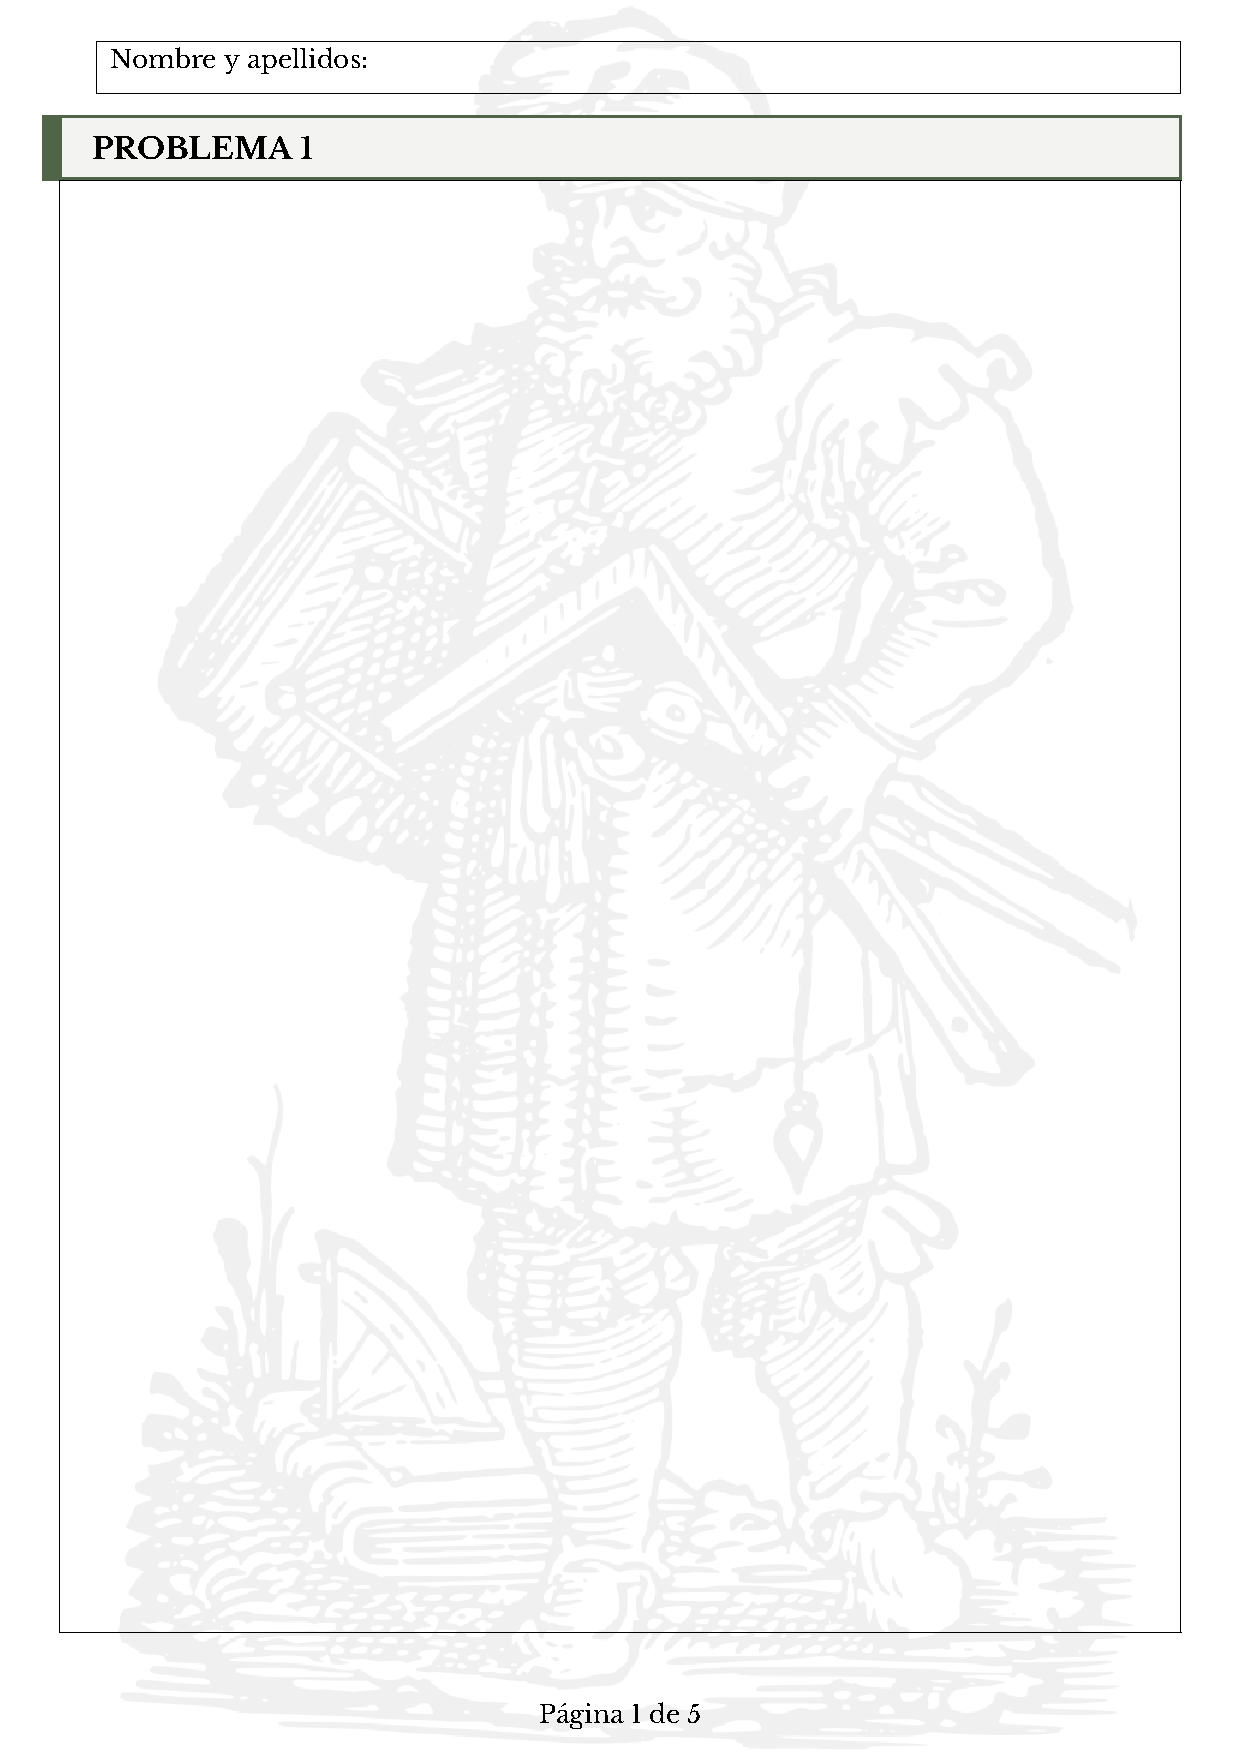
\includepdf[pages=-]{cuadernillo.pdf}
	
\end{document}